\documentclass[12pt,a4paper]{article}
\usepackage{tikz}
\usetikzlibrary{arrows, arrows.meta}
\usepackage[utf8]{inputenc}
\usepackage{amsfonts}
\usepackage{amsmath}
\newcommand{\underwrite}[3][]{% \underwrite[<thickness>]{<numerator>}{<denominator>}
  \genfrac{}{}{#1}{}{\textstyle #2}{\scriptstyle #3}
}
%\usepackage{mathptmx}
\usepackage{float}
\usepackage{graphicx}
\usepackage{multicol}
\usepackage{hyperref}
\usepackage{setspace}
\usepackage[document]{ragged2e}
\usepackage{fancyhdr}
\usepackage[left=2.5cm,right=2.5cm,top=2.5cm,bottom=2.5cm]{geometry}
\usepackage{gb4e}
\author{Tschomski}
\title{COGS542\\Grammars, Combinators and Cognition\\Lecture Notes}

\spacing{1.25}

\pagestyle{fancy}
\fancyhf{}
\lhead{Tschomski}
\rhead{COGS542}
\cfoot{\thepage}

\begin{document}\thispagestyle{empty}
\maketitle
\vspace{20pt}
\begin{center}
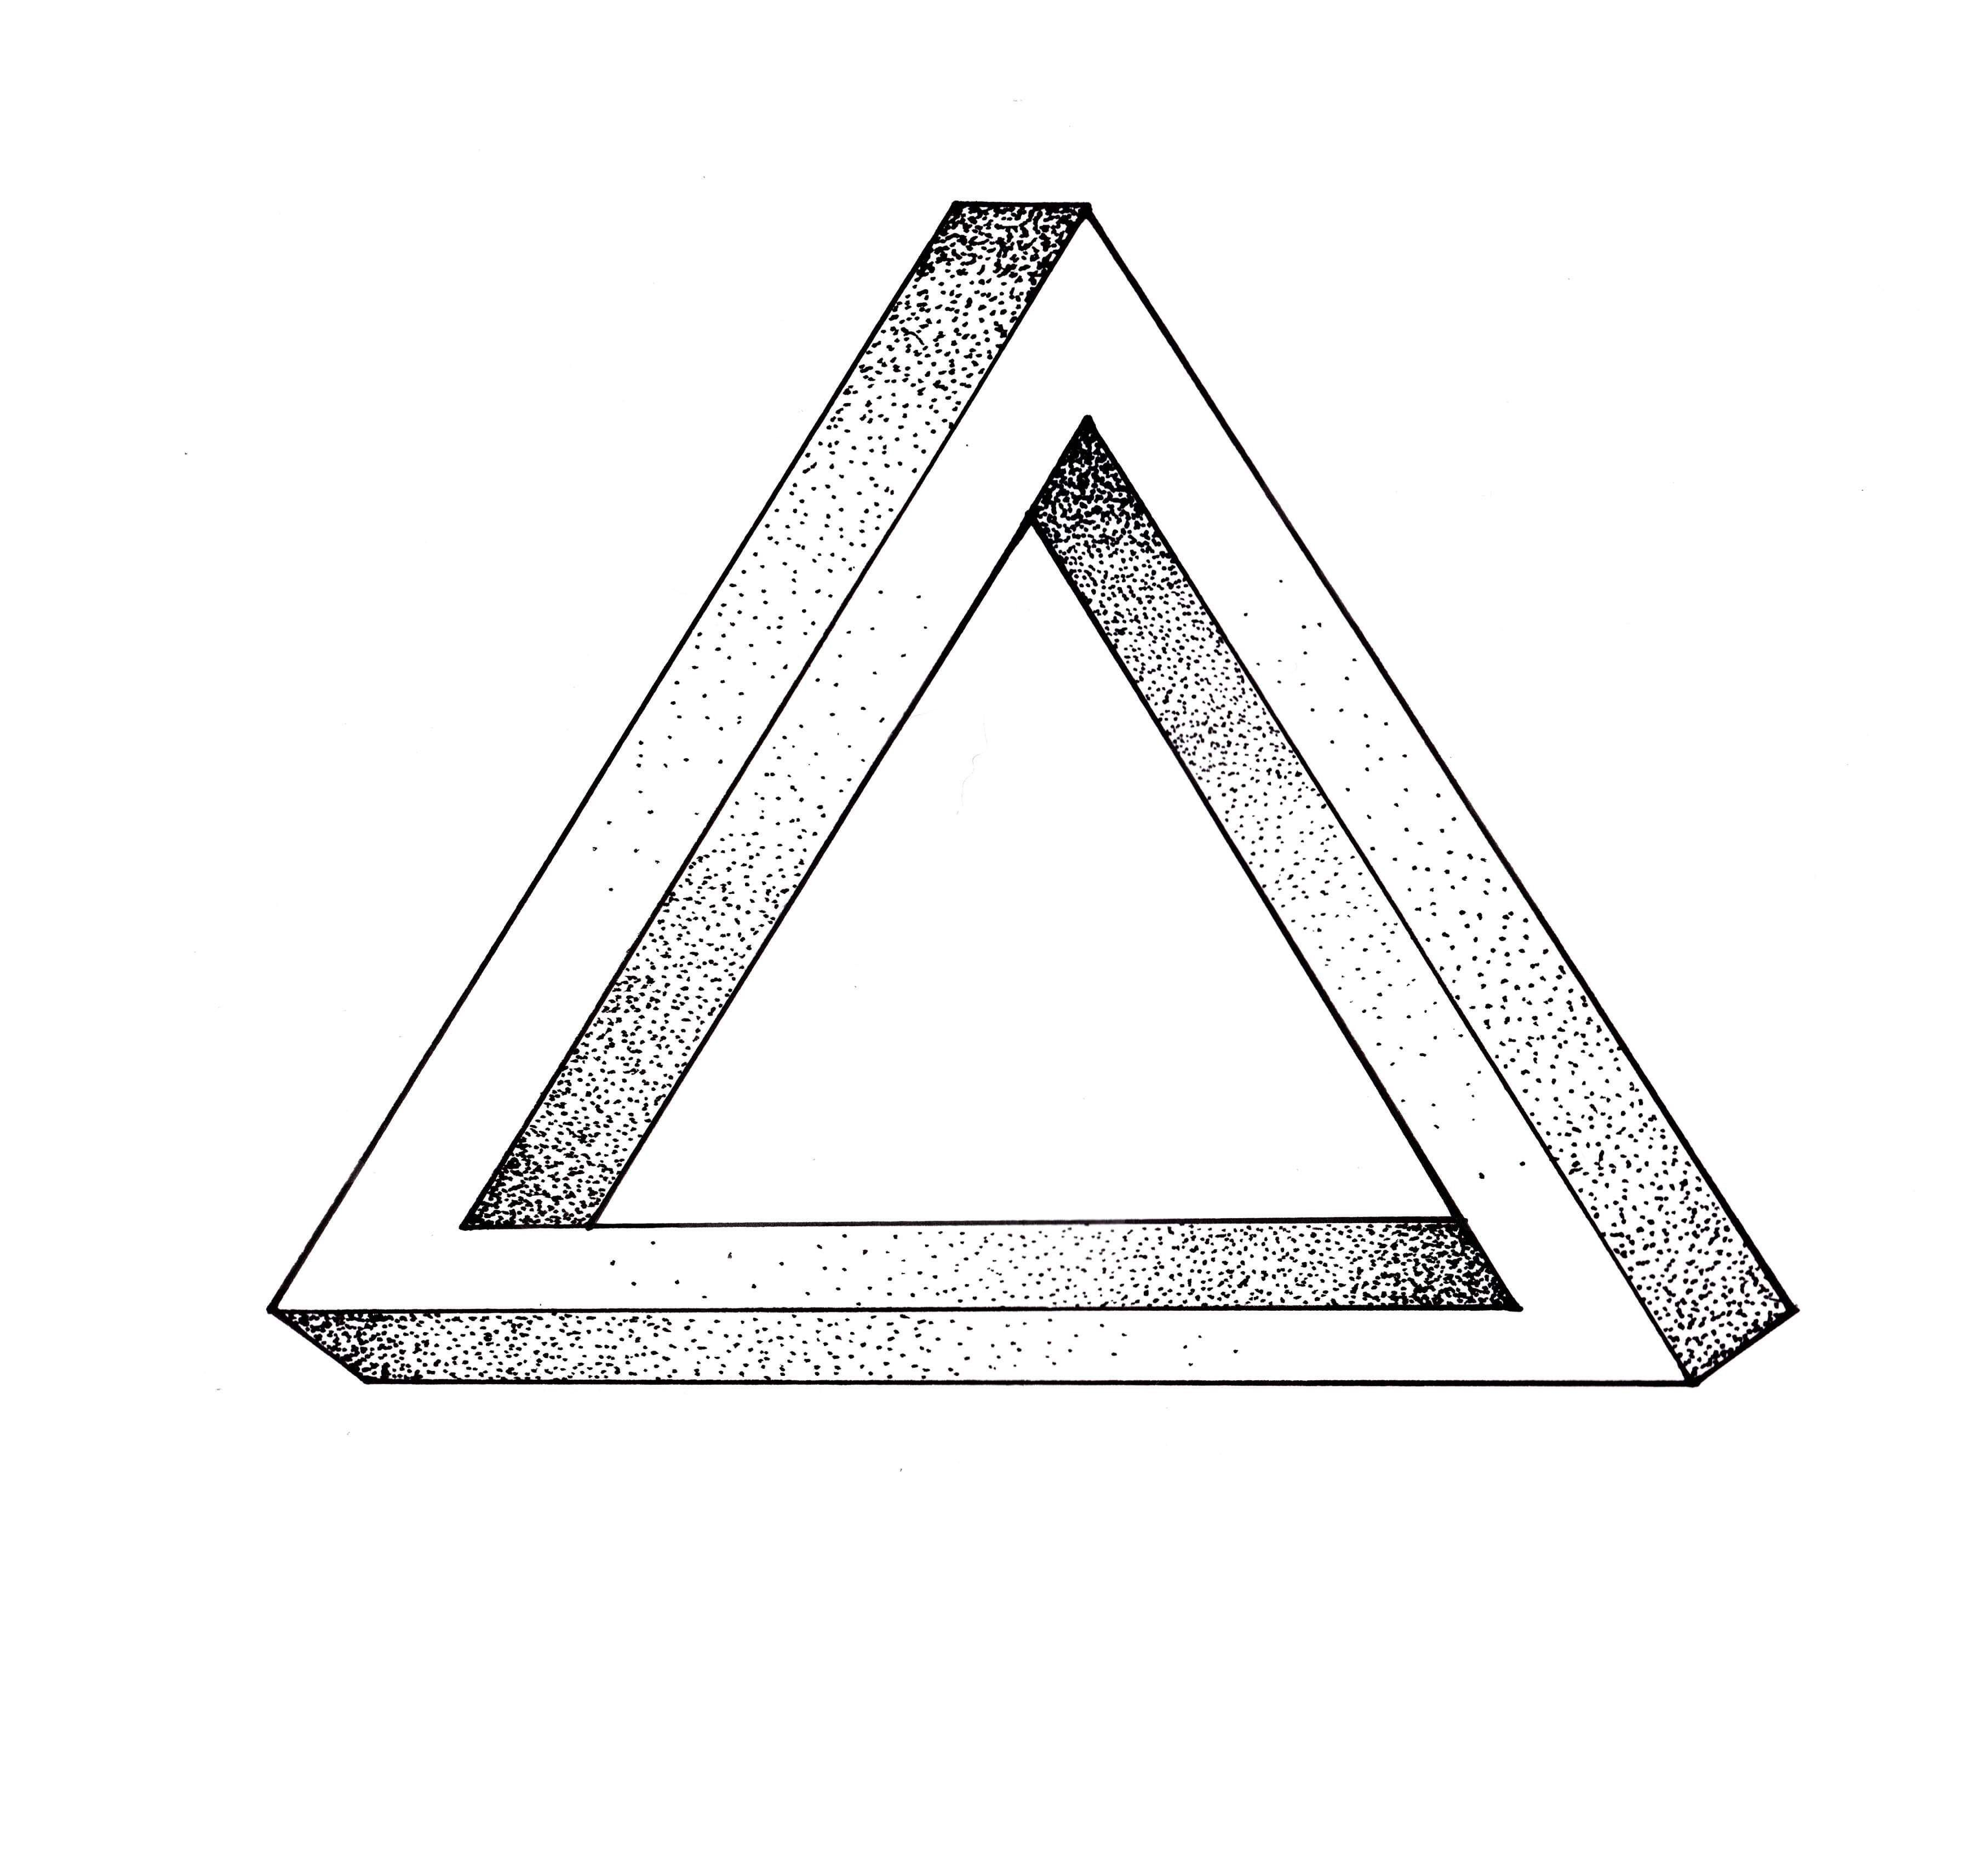
\includegraphics[scale=0.12]{ucgen}
\end{center}
\justify
\clearpage
\tableofcontents
\clearpage
\section{Introducing the Course}
Combinators and their syntax-semantics. Combinators and the lexicon. Morphology and grammar. Parsing and language acquisition. Syntactic analyses of various phenomena using combinators. Codeterminism in syntax and semantics. Combinators and serializable knowledge.
\subsection{Description of the Course}
To gain an understanding of how order and its semantics can give rise to linguistic structure. To appreciate the different implications of type-dependent and structure-dependent grammars. To build models of syntax, morphology and parsing using combinators and Combinatory Categorial Grammar. To situate combinatory theories in cognitive science including philosophy, language, music, planning and reasoning. Third of the course is about combinators and structure of meaning. Another third is about computational language models with combinators, using CCG. The last third is about combinators and plan structure, which is exploratory. The course explores the idea that planning and language may have many things in common.
\subsection{Syllabus}
\begin{table}[H]
\renewcommand{\arraystretch}{1.5}
\begin{tabular}{|c l|}
\hline
Week & Topic                                   \\ \hline
1    & Introducing the Course                  \\ \hline
2    & Introduction to Combinators 			   \\ \hline
3    & Combinators in Natural Language              \\ \hline
4    & Combinators in Natural Language (cont'd)      \\ \hline
5    & Projection of Natural Language Combinators       \\ \hline
6    & Learning the projected component's items\\ \hline
7    & Obtaining the projected component's items\\ \hline
8    & Planning                          		\\ \hline
9    & Midterm Exam                     		 \\ \hline
10   & Language of Thought             			\\ \hline
11   &        									 \\ \hline
12   & Presentations               				\\ \hline
13   &                							\\ \hline
14   &                							\\ \hline
\end{tabular}
\end{table}

\section{Introduction to Combinators}
Basic idea behind combinators is to \underline{compositionally} \underline{derive} more \underline{interpretations} of a \underline{sequence} of elements which are themselves are \underline{meaningful}. The underlined keywords are important notions in this definition in that what they are and what they mean. We need to look at these keywords in order to understand why combinators are essentially very useful understanding the cognition.  Although he cognition is very parallel in signal transmission, when it comes to high level cognitive processes such as language, vision and planning, that is all massively serial. The reason why it is serial is that it requires a kind of synchronization and coordination. When we look at ourselves, the human beings, we see that we are sequence interpretation machines, we cannot help interpreting sequences without meaningful elements in the sequence.
\subsection{What does it mean to be meaningful?}
The order of the elements and the conventions in which they are used reveal the meaning of the sequence. Look at the following sequence. 
\begin{center}
(1) $\cdots$ John buy ticket fly $\cdots$
\end{center}
This sequence can mean that John buys a ticket to fly because conventionally as the semantic properties of the elements require, one buys something since there must be a buyer and buyee, also this serves an aim. Therefore, we can extract the meaning above. Let's take a look at another sequence where the same elements are given yet in a different order.
\begin{center}
(2) $\cdots$ John fly buy ticket $\cdots$
\end{center}
In this sequence, you can derive the meaning that John wants to fly, so he buys a ticket. Depending on the order and interpretations, you begin to make different inferences for the outcome. The meaning of the sequence are updated when new conventions are included into the model. For example, considering the sequence (1), now suppose that the ticket is for a concert. In this case, the meaning that John buys a ticket for a concert and flies to where the concert takes place to use the ticket. The key point here is that different ordering of the elements leads to different interpretations and different conventions lead to different meanings despite the same order. This idea was put forward by Edmund Husserl in 1900. He said if you have a sensible distinction of meaning in a sequence, and only way you can discern that meaning difference and work with it is to have a different representation for it. This can be said to be the starting point of categorical grammar.
\subsection{What are the combinators?}
A combinator is a lambda term with no free variables. The reason why there is no free variable is that it gives you compositionality in a very rigorous way, and this is the first step understanding meaning of more and more complex sequences.
\begin{center}
(3) $\lambda x\lambda y.+$ $x$ $y$ \hspace{1cm} 
(4) $\lambda.+$ $x$ $y$
\end{center}
The lambda term in (3) is a combinator because all the variables, $x$ and $y$ are bound, and there is not free variable\footnote{The symbol, $+$ is a constant.}. However, the lambda term in (4) is not a combinator because it has a free variable, $y$. There is no binding for $y$; thus, it cannot be interpreted compositionally. Now let's take a look at the sequence $\cdots$ mother father $\cdots$. This sequence means that \emph{``mother of father"}. Therefore, we can define two lambda terms as in (5) and (6).
\begin{center}
(5) mother = $\lambda x.mother$ $x$ \hspace{1cm}
(6) father = $\lambda x.father$ $y$
\end{center}
Using these lambda terms, we can find mother of father of someone as in (7). This is what we call function composition in mathematics.
\begin{center}
(7) $\lambda z.mother(father$ $z)$
\end{center} 
However, there is a combinatory way of writing this without introducing any variables into the sequence. This is where we introduce combinators.
\begin{itemize}
  \item[] $\textbf{\textsf{B}} \overset{def}{=} \lambda f\lambda g\lambda x.f(gx)$ (compositor)
  \begin{itemize}
  \item[$\equiv$]$\cdots$ \textbf{\textsf{B}} mother father $\cdots$
  \item[$\rightarrow$] In the lambda terms given above, the two terms are not related to each other, but when combinator \textbf{\textsf{B}} is used, the terms get a meaning together. This is the use of combinators.
  \end{itemize}
  \item[] $\textbf{\textsf{S}} \overset{def}{=} \lambda f\lambda g\lambda x.fx(gx)$ (substitutor)
  \begin{itemize}
  \item[] $\cdots$ the books I have read without understanding $\cdots$
  \item[] $(\lambda x.not-understand$ $x(read$ $x))books$ 
  \end{itemize}
  \item[] $\textbf{\textsf{W} }\overset{def}{=} \lambda f\lambda x.fxx$ (duplicator)
  \begin{itemize}
  \item[] $\cdots$ John turn  $\cdots$ \textit{(Take the argument and copy it!)}
  \item[] \textbf{\textsf{W}}.turn John $\rightarrow$ John turn John (himself)
  \end{itemize}
  \item[] $\textbf{\textsf{C}} \overset{def}{=} \lambda f\lambda g\lambda x.fxg$ (permutator)
  \item[] $\textbf{\textsf{I}} \overset{def}{=} \lambda x.x$ (identificator)
  \begin{itemize}
  \item[] $\cdots$ \textbf{\textsf{C I}} John turn $\cdots$ \textit{(Take the sequence and change the order of the last two!)}
  \item[] $\cdots$ \textbf{\textsf{I}} turn John $\cdots$ \textit{(Take the argument and give it back as it is!)}
  \item[] $\cdots$ turn John $\cdots$
  \end{itemize}
  \item[] $\textbf{\textsf{K}} \overset{def}{=} \lambda f\lambda g.f$ (cancellator)
  \item[] $\textbf{\textsf{T}} \overset{def}{=} \lambda f\lambda g.gf$ (commutator)
\end{itemize}
\vspace{1cm}

\textbf{\Large{QUIZ 1:}}\\

\textbf{Question:} Show that \textsf{BSC=B(BW)B}.\\

\noindent \textit{\textbf{Hint:} Combinators are lambda terms; therefore, they apply the same way using function application (i.e. beta reduction). Recall that '=' is an extensional concept in this world. Two things are equal if they behave the same in arbitrary choice of elements. For example, M=N if and only if Ma = Na for arbitrary a.}\\
\textit{What all this means is that for example $Babc=a(bc)$, because $B=(\lambda f\lambda g\lambda x.f(gx))$, and $(\lambda f\lambda g\lambda x.(gx))abc=a(bc)$.}\\
\textit{Another example: $BKabc=ab$ because $BKabc=K(ab)c=ab$.} \\

\textbf{Answer:} Feeding both combinators with the same elements, x, y and z;

\begin{multicols}{2}
\begin{itemize}
\item[=]\textsf{BSC}xyz
\item[=]\textsf{S}(\textsf{C}x)yz
\item[=](\textsf{C}x)z(yz)
\item[=]x(yz)z
\end{itemize}

\columnbreak

\begin{itemize}
\item[=]\textsf{B(BW)B}xyz
\item[=]\textsf{(BW)(B}x)yz
\item[=]\textsf{W((B}x)y)z
\item[=]((\textsf{B}x)y)zz
\item[=]x(yz)z
\end{itemize}

\end{multicols}

\clearpage

\section{Combinators in Natural Language}
Combinators are essentially mathematical objects, and the empirical domain of ontology for sequences you have such as sequences of actions and words etc. shows how combinatory theory for those will be dealing with their problems. Combinators tell what is possible and what is not in these empirical domains. Since the most worked out domain for combinators is natural language, combinators in natural language will be covered in this section. To introduce the notation in combinatory categorial grammar (CCG), let's see the following natural language string in (1).

\begin{exe}
		\ex
			\begin{xlist}
				\gll a. John likes Mary $\rightarrow$ Observable\\
				b. NP (S$\setminus$NP)/NP NP\\
				c. $John'$ $\lambda x\lambda y.likes'xy$ $Mary'$
			\end{xlist}
	\end{exe}
	
(1a) indicates the observables in other words the phonological elements on the surface. (1c) shows the predicate argument structure of $like$. Lambda terms in (1c) point out the prominence in that subjects are more prominent than direct objects, direct objects are more prominent than indirect objects and beneficiaries etc. Therefore, in natural language, arguments of predicates have relative prominence. The meanings of the observables come from the predicate argument structures of the lambda terms and the life-time experience on these elements. The issue here combinators do not tell anything about the order of the elements. To resolve this problem, some kind of a directionality can be put forward. In this directionality notation (/) means predicate needs an arguments to its right and ($\setminus$) means predicate needs an argument to its left. In (1b), the phrase, $S$ needs an argument to its left which is $NP$, John and to its right which is $NP$, Mary. The CCG notation for (1) is as follows:\\

(2) $\underwrite{\text{$likes' :=$}}{Phonological Element}\ 
  \underwrite{\text{(S$\setminus$NP)/NP:}}{Syntactic Type}\ 
  \underwrite{\text{$\lambda x\lambda y.likes'xy$}}{Logical Form}$\\

This is how the sequences are represented showing their order and meaning. The drawing notation for this representation is as follows (FA means \textit{Function Application}):\\
 
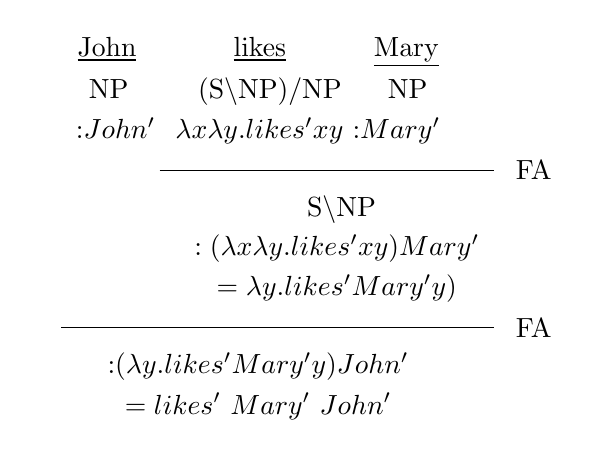
\begin{tikzpicture}
\node at (0,0) {\underline{John} \hspace{1cm} \underline{likes}\hspace{1cm} \underline{Mary}};
\node at (0,-0.5) {NP \hspace{0.65cm} (S$\setminus$NP)/NP \hspace{0.35cm} NP};
\node at (0,-1) {:$John'$ \hspace{0.02cm} $\lambda x\lambda y.likes'xy$ :$Mary'$};
\draw (-1.25,-1.5) -- (3,-1.5);
\node at (3.5,-1.5) {FA};
\node at (0,-2){\hspace{2cm} S$\setminus$NP};
\node at (0,-2.5){\hspace{2cm}$:(\lambda x\lambda y.likes'xy)Mary'$};
\node at (0,-3){\hspace{2cm}$=\lambda y.likes'Mary'y)$};
\draw (-2.5,-3.5) -- (3,-3.5);
\node at (3.5,-3.5){FA};
\node at (0,-4){:$(\lambda y. likes' Mary'y)John'$};
\node at (0,-4.5){$=likes'$ $Mary'$ $John'$};
\end{tikzpicture}

As can be seen having an argument on the right is function application and also having an argument to the left is function application as well.
\begin{itemize}
\item[] $\alpha := X/Y:f$ $\beta :=Y:a$ $\rightarrow$ $\alpha\beta :=X:fa$ (Forward Application)
\item[] $\alpha := Y:a$ $\beta :=X\setminus Y:f$ $\rightarrow$ $\alpha\beta :=X:fa$ (Backward Application)
\item[] We can write as $X/Y$ $Y$ $\rightarrow$ $X$ ($>$) and $Y$ $X\setminus Y$ $\rightarrow$ $X$ ($<$).
\end{itemize}

These notations are the common usage in many CCG papers, and although it seems to do a sort of syntactic ordering, these rules do phonology, syntax and semantics all in a single computation, which the beauty of CCG.

The question here is why we need B and S combinators in CCG if all we do is function application. That is where things begin to get more interesting. Let's remember the lambda terms regarding the combinators B and S below:

\begin{itemize}
\item[] $B=\lambda f\lambda g\lambda x.f(gx)$ \hspace{1cm} $S=\lambda f\lambda g\lambda x.fx(gx)$
\end{itemize}

Take the sequence w_{1}w_{2}w_{3}, their function composition and meanings. Through combinators, we get phonology, syntax and semantics of the elements all together. All functions are curried (schönfinkeled). Therefore, the function composition is going to look like below given in curried form.\\

\begin{tabular}{ccccc}
Sequence: & w_{1} & w_{2} & w_{3} & w_{1}w_{2}w_{3} \\
    (B)   & X/Y   & Y/Z   & Z     & $\rightarrow$ X    \\
Meaning:        & $:f$    & $:g$    & $:x$    & $:f(gx)$ \\ \hline
\end{tabular}\\

\textbf{In curried form:} $X/Y:f$ $Y/Z:g$ $\rightarrow$ $X/Z:\lambda x.f(gx)$\\

\begin{tabular}{ccccc}
Sequence: & w_{1}   & w_{2} & w_{3} & w_{1}w_{2}w_{3}  \\
(S)       & (X/Y)/Z & Y/Z   & Z     & $\rightarrow$ X     \\
Meaning:          & $:f$      & $:g$    & $:x$    & $:fx(gx)$ \\ \hline
\end{tabular}\\

\textbf{In curried form:} $(X/Y)/Z:f$ $Y/Z:g$ $\rightarrow$ $X/Z:\lambda x.fx(gx)$\\

\begin{tabular}{ccccc}
Sequence: & w_{1}   & w_{2} & w_{1}w_{2}  \\
(T)       & Y & X/Y   & $\rightarrow$ X     \\
Meaning:          & $:a$      & $:b$   & $:ba$ \\ \hline
\end{tabular}\\

\textbf{In curried form:} $Y:a$ $X/Y:b$ $\rightarrow$ $X:ba$\\

\subsection{Function Application}
The use of combinators is different from function application. What is done by function application is to give the functions their arguments and incrementally process them. Let's, for example, rewrite the combinator, $T$ by taking $X/Y$ to the right in $X/Y:b$ $Y:a \rightarrow X:ba$.\\

$Y:a \rightarrow X \setminus (X/Y):\lambda p.pa$\\

\noindent This process is called \textbf{type-raising}, and it is not the projective component unlike the combinators because it is not order-preserving. The notation given above is forward application as well. If you want to see backward application, it is going to look like as follows:\\

$Y:a \rightarrow X \setminus Y:b \rightarrow X:ba$\\

\noindent If we want to move the function, we are going to get the following:\\

$Y:a \rightarrow X/(X\setminus Y):\lambda p.pa$\\
\subsection{What is projected by the combinatory projection?}
So far, it has been shown that the combinators deal with syntax, semantics and phonology at the same time in combinatory surface calculus. However, to appreciate their real power, we need to have some real empirical data to test all the theory put forward by CCG. For example, take the sentence, John likes Mary.\\

\begin{tabular}{ccccc}
Example: & \underline{John}   & \underline{likes} & \underline{Mary}  \\
         & $NP:j'$ & $(S\setminus NP)/NP$   & $NP:m'$     \\
         &         & $\lambda x\lambda y.likes'xy$   &  \\ \hline
\end{tabular}\\

And when we do the function applications, we get:
\begin{itemize}
\item[]$=(\lambda x\lambda y.likes'xy)m'$
\item[]$=\lambda y.likes'm'y$
\item[]$=(\lambda y.likes'm'y)j'$
\item[]$=likes'm'j'$
\end{itemize}

\vspace{1cm}

\textbf{\Large{QUIZ 2:}}\\

\textbf{Question:} We can take the combinator $W$ and try to symbolize it, just like I did for $B$ and $S$. For simplicity, I will again assume that in its definition, $W=\lambda f\lambda x.fxx$, we are always looking forward in a sequence. So we get: $(X/Y)/Y:f$ $Y:x$ $\rightarrow$ $X:fxx$\\

Why? Because $f$ is a two argument function, and arguments are identical, hence $X/Y/Y$ rather than $X/Y$. Also, there is one input $x$ to $W$, so we don't have $X/Y/Y$ $Y$  $Y$ $\rightarrow$ $X$, because that would mean three inputs to $W$.\\

After this introduction, try the same process for $C=\lambda x\lambda y\lambda z.xzy$ for the quiz. Note that $W$ is already a two-input combinator, but $C$ is not. So I suggest you first write the $C$ as I did for $B$ and $S$ for all its inputs, then \textit{``curry"} the result so that it creates a partial function, much like I did for $B$ and $S$.\\

\noindent \textbf{Answer:} Unlike the combinator $W$, $C$ takes two arguments, and neither of these arguments are a function in contrary to the combinator $B$ and $S$. Therefore, we can have singular expressions like $Y$ and $Z$ (not like $Y/Z$) for the arguments as given below.\\

\begin{tabular}{ccccc}
Sequence: & w_{1}   & w_{2} & w_{3} & w_{1}w_{2}w_{3}  \\
(C)       & (X/Y)/Z & Y   & Z     & $\rightarrow$ X     \\
Meaning:          & $:x$      & $:y$    & $:z$    & $:xzy$ \\ \hline
\end{tabular}\\

\textbf{In curried form:} $(X/Y)/Z:x$ $Y:y$ $\rightarrow$ $X/Z:\lambda z.xzy$\\

\textbf{\Large{QUIZ 3:}}\\

\textbf{Question:} Take the following English expression, \textit{the book that Mary quickly read}. Here ``read" cannot be the transitive ``read". It is a two-argument function. We are concerned about how to obtain the following combinations:\\

the book that[Mary[quickly read]].\\

\noindent By assigning categories to words in brackets, show how we can obtain the bracketed grouping using $B$ and $T$. Method is to assign categories to three words in the brackets. Each category must contain a syntactic type and a lambda term, representing roughly its meaning. For example, we have $the:=NP/N: \lambda x.def'x$ and $book:=N:book'$. We are only interested in obtaining the bracketed string. You don't need to show how it combines with `the', `book', and `that'.

\noindent \textbf{Answer:}\\

\begin{tabular}{ccccc}
pho: & \underline{Mary}  & \underline{quickly} & \underline{read} & \\
syn: & $NP$  & $Adv/VP$   & $(VP\setminus NP)/NP$ & \\
sem: & $mary'$ & $\lambda f.quickly' f$    & $\lambda x \lambda y.read'xy$ & $FA$  \\ \cline{3-4}
\end{tabular}\\

\hspace{3cm} $(Adv\setminus NP)/NP$

\hspace{3cm} $quickly'(\lambda x \lambda y.read'xy)$\\
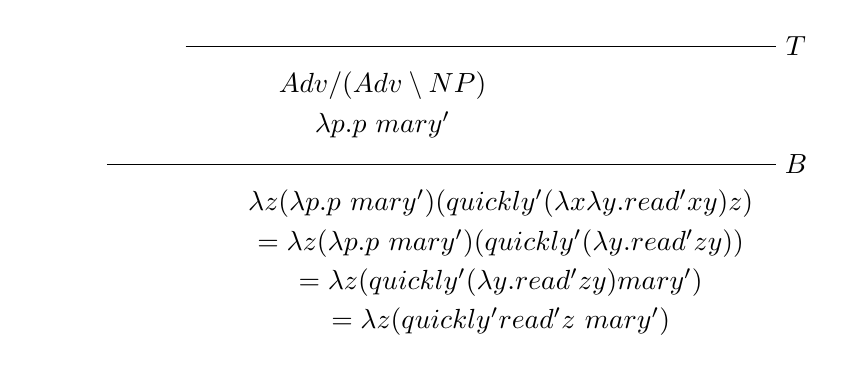
\begin{tikzpicture}
\draw[white] (0,0) -- (2,0);
\draw (2,0) -- (9.5,0);
\node at (4.5,-0.5) {$Adv/(Adv\setminus NP)$};
\node at (4.5, -1) {$\lambda p.p$ $mary'$};
\node at (9.75, 0) {$T$};
\draw[white] (0,-1.5) -- (1,-1.5);
\draw (1,-1.5) -- (9.5,-1.5);
\node at (9.75, -1.5) {$B$};
\node at (6,-2) {$\lambda z(\lambda p.p$ $mary')(quickly'(\lambda x \lambda y.read'xy)z)$};
\node at (6,-2.5) {$=\lambda z(\lambda p.p$ $mary')(quickly'(\lambda y.read'zy))$};
\node at (6,-3) {$=\lambda z(quickly'(\lambda y.read'zy)mary')$};
\node at (6,-3.5) {$=\lambda z(quickly'read'z$ $mary')$};
\end{tikzpicture}\\

First, in the derivation, function application is done to form the main function which is \textit{``quickly read"} because this is going to take the arguments (I have made this choice since \textit{``quickly"} cannot stand alone and it acts as a single unit with \textit{``read"}). Then, to merge \textit{``Mary"} into the derivation, the combinator, $T$ is used as the function is looking for something to its right first, but ``Mary" is on the left. Thus, type-raising is applied here. Finally, since \textit{``read"} is a transitive verb, yet here it seems to be intransitive (in fact it is not) as its argument happens to be somewhere else for now (We are not concerned with it right now). Therefore, to make its merge into the derivation, the combinator $B$ is used ($z$ will be replaced by \textit{``the book"}). By this way, the expression \textit{``the book that Mary quickly read"} is derived from its base form (?) \textit{``Mary quickly read the book"}.
\clearpage
\section{Projection of Natural Language Combinators}
In natural language combinators, the directionality is of great importance.
\begin{itemize}
\item[$(>B)$ ] \hspace{1cm} $X/Y:f \hspace{1cm} Y/Z:g \rightarrow X/Z:\lambda x.f(gx)$
\item[$(>B_\times)$] \hspace{1cm} $X/Y:f \hspace{1cm} Y\setminus Z:g \rightarrow X\setminus Z:\lambda x.f(gx)$ (forward crossing composition)
\item[$(<B_\times)$] \hspace{1cm} $Y/Z:g \hspace{1cm} X\setminus Y:f \rightarrow X/Z:\lambda x.f(gx)$ (backward crossing composition)
\item[$(<B)$ ] \hspace{1cm} $Y\setminus Z:g \hspace{1cm} X\setminus Y:f \rightarrow X\setminus Z:\lambda x.f(gx)$ (backward harmonic composition)
\item[$(>S)$ ] \hspace{1cm} $X/Y/Z:f \hspace{1cm} Y/Z:g \rightarrow X/Z:\lambda x.fx(gx)$
\item[$(<S)$ ] \hspace{1cm} $Y/Z:g \hspace{1cm} X/Y/Z:f \rightarrow X\setminus Z:\lambda x.fx(gx)$
\item[$(>S_\times)$] \hspace{1cm} $(X/Y)\setminus Z:f \hspace{1cm} Y\setminus Z:g \rightarrow X\setminus Z:\lambda x.fx(gx)$
\item[$(<S_\times)$] \hspace{1cm} $Y/Z:g \hspace{1cm} (X\setminus Y)/Z:f \rightarrow X/Z:\lambda x.fx(gx)$
\item[$(>T)$ ] \hspace{1cm} $X:a \rightarrow T/(T\setminus X):\lambda p.pa$
\item[$(<T)$ ] \hspace{1cm} $X:a \rightarrow T\setminus(T/X):\lambda p.pa$
\end{itemize}

\subsection{Projection Principle of CCG}
Everything in the lexicon is projected onto surface structures unchanged, undeleted and unmoved.

32.10dan devam et.



































\end{document}